\documentclass{article}
\usepackage[dblblindworkshop]{neurips_2026}
\workshoptitle{The Third Workshop on Agents in the Wild: Safety, Security, and Beyond}
\usepackage[utf8]{inputenc}
\usepackage[T1]{fontenc}
\usepackage{hyperref}
\usepackage{url}
\usepackage{booktabs}
\usepackage{graphicx}
\usepackage{enumitem}

\title{The Chain Is Signed, the Handoff Is Prose:\\Measuring Provenance Loss at the Model Layer}

\author{%
  Anonymous \\
}

\begin{document}
\maketitle

\begin{abstract}
Capability-based delegation already solves provenance. UCAN describes its delegation chain as
``by definition a provenance log''; RFC~8693 encodes an ordered actor chain in nested \texttt{act}
claims; ZCAP-LD, and the 2026 agent-specific proposals built on them, extend this to multi-hop
agent delegation. None of that is in dispute. The gap is elsewhere: the signed chain lives in a
token envelope the language model never reads, and the handoff the model actually writes is prose.
We measure what that prose carries. Across 480 delegation chains and 1{,}440 generation hops on
four model families, a principal's identity survives to the end of an unprompted chain in
\textbf{35.8\%} of cases. One explicit instruction to carry identity forward raises this to
\textbf{99.6\%}. Three results are more useful than the headline. First, loss is not gradual: 52.5\%
of depth-5 chains have already lost full provenance after the \emph{first} handoff, and only 15
further points are lost over the four hops that follow. Second, model family dominates depth: unprompted
preservation ranges from 5.0\% to 90.0\% across families, an 85-point spread that the instruction
collapses to under 2. Third, the instruction is the \emph{only} arm that fabricates. Zero of 240
control chains invent an identity; 2 clause chains invent a delegating persona, because an
instruction to preserve received attributions gives a model no way to distinguish a true
attribution from one an earlier hop hallucinated. A signed chain rejects an unsigned link; prose
has no such check. We therefore read the clause not as a fix but as a measured floor, and its
residual failures as the argument for the cryptographic layer.
\end{abstract}

\section{The gap that is actually open}

When an agent delegates to a sub-agent, who is the work being done for? At the token layer this is
answered. UCAN calls its chain ``by definition a provenance log''~\citep{ucan}. RFC~8693 token
exchange nests an ordered \texttt{act} claim so that, in its own words, a chain of delegation
forms ``a history trail that connects the initial request and subject through the various
delegation steps''~\citep{rfc8693}. ZCAP-LD provides capability-based authority with
cryptographic delegation~\citep{zcap}. Agent-specific work extends these to multi-hop agent
settings: AIP fuses identity, attenuated authorization and provenance binding into an
append-only token chain spanning MCP and A2A, and rejects 600 of 600 attacks including audit
evasion~\citep{aip}; Agentic JWT, SAGA and InterSAGE build comparable delegation
machinery~\citep{agenticjwt,saga,intersage}. Survey work names the failure modes precisely,
listing
recursive delegation accountability and agent identity integrity among five gaps that no
current instrument resolves~\citep{aiidentity}.

So the standards are not the problem, and a paper claiming they are would be wrong. The problem is
that these mechanisms sit \emph{beside} the model rather than inside it. In deployed agent
frameworks the message passed between agents is natural language the model composes. The Model
Context Protocol requires that a server ``MUST NOT pass through the token it received from the
MCP client'', and names the consequence, ``Accountability and Audit Trail Issues'', without
resolving it at the message layer~\citep{mcp}. The Agent2Agent specification states plainly that
its payloads ``don't carry user or client identity information directly'', placing identity in
the HTTP layer instead~\citep{a2a}. Sub-agent frameworks pass a handoff message the model
writes.

Figure~\ref{fig:arch} shows the two layers. The cryptography is intact and unused at the point where the model decides what to say next. That
decision is measurable, and to our knowledge has not been measured. AIP reports verification
latency and adversarial rejection rates but no measurement of what a model actually writes in a
handoff~\citep{aip}; the gap analyses run no experiments at all~\citep{aiidentity}. Every
protocol result we are aware of places enforcement outside the model.

This matters for deployed systems specifically because the failure is silent. A delegation whose
prose has dropped the principal still completes, still returns a plausible result, and still
leaves a well-formed signed chain in the token envelope. Nothing errors. An operator reading the
envelope sees an intact audit trail; an operator reading what the agents actually said to each
other sees, in the median unprompted configuration, no principal at all. Our aim is to say how
far apart those two views are, and under what conditions they diverge.

\section{Method}

A task is issued by a named principal, for example ``Priya Raghavan, employee ID E-4471,
Finance''. Agent~1 receives it, does part of the work, and writes a natural-language handoff to
Agent~2. Agent~2 sees \emph{only} that handoff, not the original task, and delegates onward. We run
chains of depth 1, 3 and 5.

Two arms. \textbf{Control}: the system prompt describes the delegation task and says nothing about
identity. \textbf{Clause}: the same prompt plus one instruction, that the handoff must state on
whose behalf the work is performed, including name and identifier, and must preserve any such
statement received.

The dependent variable is whether the terminal handoff still names the originating principal:
\textsc{full} (name and identifier), \textsc{partial} (one of the two), \textsc{lost} (neither).
We also flag chains that assert an identity other than the true principal.

Four families on AWS Bedrock: Claude Haiku~4.5, Llama~3.3~70B, Nova~Pro, Pixtral~Large.
Twenty independent chains per family $\times$ arm $\times$ depth cell, so $4\times2\times3\times20
= 480$ chains and 1{,}440 hops, with zero parse failures. Scoring is programmatic first, by string
match on surname and normalised identifier; a Claude judge scores every chain independently and
flags fabrication. The two agree on 479 of 480 chains (99.8\%), and we report both. Total cost
was USD~2.32 at list prices.

The harness also computes a cheap regular-expression screen for fabricated identifiers, which
flags any token shaped like an employee ID that is not the true principal's. We disclose it
because we do \emph{not} use it. It fires on 25 of 480 chains against 2 confirmed, a precision
of 0.04, matching strings such as \texttt{ISO 27001} and \texttt{all 824}; and it misses the
fabrication that invents a name but no identifier, a recall of 0.50. Every fabrication figure
we report comes from the judge, which ran on all 480 chains and not on a screened subset.

\section{Results}

\begin{figure}[t]
\centering
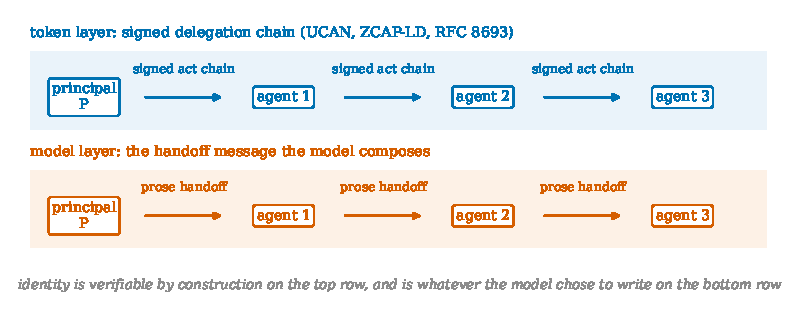
\includegraphics[width=\textwidth]{p1_arch.pdf}
\caption{The two layers. Capability-based delegation records an ordered, verifiable chain of
principals in the token envelope (top). The message the model actually composes and passes to
the next agent is prose (bottom), and the model never reads the envelope. We measure what the
prose carries.}
\label{fig:arch}
\end{figure}

\begin{figure}[t]
\centering
\begin{minipage}[b]{0.505\textwidth}
\centering
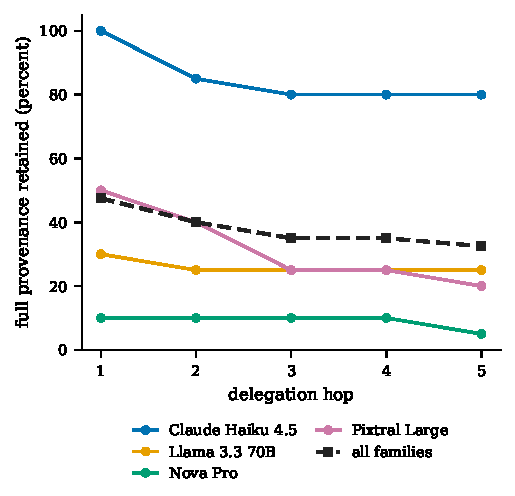
\includegraphics[width=\linewidth]{p2_perhop.pdf}
\caption{Depth-5 control chains retaining full provenance after each hop. The drop is
concentrated at the first handoff; family separates far more than hop does.}
\label{fig:perhop}
\end{minipage}\hfill
\begin{minipage}[b]{0.475\textwidth}
\centering
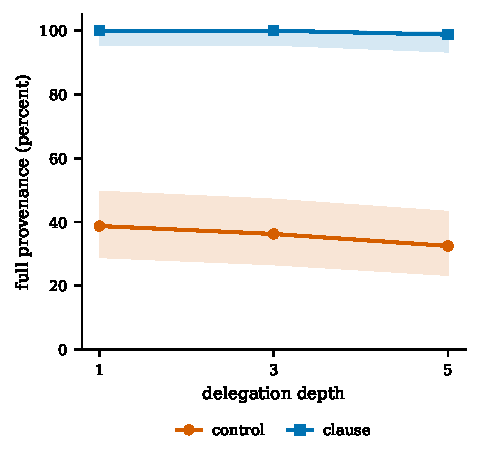
\includegraphics[width=\linewidth]{p3_armdepth.pdf}
\caption{Terminal full-provenance rate by arm and depth, pooled over families, with Wilson
95 percent bands. $n=80$ per point, 480 chains in total.}
\label{fig:armdepth}
\end{minipage}
\end{figure}

\paragraph{The clause works, and depth is not the story.}
Pooled over depths, control preserves full provenance in 86 of 240 chains (35.8\%) and the clause
in 239 of 240 (99.6\%). At depth~5 the figures are 32.5\% [23, 43] and 98.8\% [93, 100]. The
intervals are nowhere close to overlapping at any depth.

But the decline with depth is shallow: 38.8\%, 36.2\%, 32.5\% at depths 1, 3, 5. The per-hop curve
in Figure~\ref{fig:perhop} explains why. Of 80 depth-5 control chains, 42 had already lost full
provenance after the first handoff; only 12 more were lost across the remaining four hops
(retention 47.5, 40.0, 35.0, 35.0, 32.5 percent). Provenance is not eroded by repetition. It is
dropped or kept at the first paraphrase, which means depth sweeps measure the wrong axis.

\paragraph{Family dominates.}
Unprompted preservation differs by 85 points across families (Table~\ref{tab:fam}): Claude Haiku
90.0\%, Pixtral 28.3\%, Llama 20.0\%, Nova~Pro 5.0\%. Under the clause all four reach 98.3\% or
better. Any single pooled claim that agents lose provenance at some rate is therefore an artefact
of the model mix, not a property of agent delegation.

Name and identifier also dissociate, in opposite directions by family. Llama retains the bare
identifier more often than the name (30.0\% against 20.0\%), producing terminal handoffs that read
``\ldots for employee ID E-3915, Security'' with no person attached. Pixtral does the reverse
(41.7\% name against 31.7\% identifier). Reporting a single preservation figure hides which half
survived, and an identifier without a name is not usable for an audit.

\begin{table}[t]
\centering\small
\caption{Preservation by family, pooled over depths ($n=60$ per cell). Programmatic strict scoring.}
\label{tab:fam}
\begin{tabular}{lrrr rrr}
\toprule
& \multicolumn{3}{c}{\textbf{control}} & \multicolumn{3}{c}{\textbf{clause}} \\
\cmidrule(lr){2-4}\cmidrule(lr){5-7}
Family & full & name & id & full & name & id \\
\midrule
Claude Haiku 4.5 & 90.0 & 93.3 & 91.7 & 100.0 & 100.0 & 100.0 \\
Pixtral Large    & 28.3 & 41.7 & 31.7 &  98.3 & 100.0 &  98.3 \\
Llama 3.3 70B    & 20.0 & 20.0 & 30.0 & 100.0 & 100.0 & 100.0 \\
Nova Pro         &  5.0 &  5.0 &  6.7 & 100.0 & 100.0 & 100.0 \\
\bottomrule
\end{tabular}
\end{table}

\paragraph{The mitigation introduces the failure it prevents.}
Across 240 control chains, no chain invented a principal name or an identifier. Every fabrication
is in the clause arm, and both are Pixtral: 2 of 480 chains, or 2 of the 240 clause chains
(0.8\%). The mechanism is
straightforward. The control arm has no reason to assert an identity, so it omits. The clause tells
the model to assert one, and a weaker model sometimes asserts one it has produced itself.

The instances are instructive because the true principal is usually still there. What is invented
is an \emph{intermediary}. In one depth-1 chain the true principal Elena Kovalenko, E-4108, is
correctly carried, prefixed by a delegating agent who does not exist:

\begin{quote}\small
``This is now Alexei Popov on behalf of Elena Kovalenko, employee ID E-4108, Regulatory Affairs.''
\end{quote}

The second, at depth~5, is the more instructive of the two, because the real principal has been
flanked by two invented ones carrying well-formed identifiers:

\begin{quote}\small
``On behalf of Aidan Xu, employee ID E-5175, Naomi Okonkwo, employee ID E-6124, and Alex Lorenz,
employee ID E-1234, in Finance: Gather all additional documents required by the checklist.''
\end{quote}

Only Naomi Okonkwo, E-6124, is real. Both scorers mark this chain \textsc{full}, correctly, since
the true principal is present and correctly identified. Preservation and fabrication are
orthogonal, and a preservation metric on its own would record this chain as a success. The clause
says to preserve any attribution received, and prose offers no way to distinguish an attribution
that arrived legitimately from one a previous hop invented. A signed chain rejects an unsigned
link; a sentence does not.

\section{What we conclude}

We do not claim a spec clause fixes provenance. It raises a measured rate from 35.8\% to 99.6\%,
which is a floor worth having, and it introduces a low-rate accretion failure that the
cryptographic layer exists to catch. The argument that prompt- and training-level identity
guarantees are only probabilistic, since stochastic reasoning and multi-agent orchestration can
silently expand what an agent asserts~\citep{agenticjwt}, is on this evidence correct. Our contribution is to put a
number on the probability, and to show the residual failures are exactly the ones a verifiable
chain rejects by construction. That makes the two layers complementary rather than competing:
prose carries intent, tokens carry authority, and a system that relies on prose for authority is
relying on a 35.8\% mechanism.

\paragraph{Reporting.} For any agent system claiming an audit trail, report the terminal
provenance rate per model family and not pooled, report name and identifier separately, and report
the hop-1 rate, since that is where the loss occurs.

\paragraph{Limitations.} One task domain and one prompt template; the phrasing of the clause is
plainly a free variable we did not sweep. Preservation is measured on what the model \emph{says},
which is the point, but it is not evidence about the enforcement layer. Four families, one of them
substituted after two Claude model identifiers were unavailable to this account. Fabrication rests
on 2 events and its rate should be read as an existence proof, not an estimate. All chains are
synthetic, and a real deployment carries system-level identity the model may see through other
channels.

\paragraph{Artefacts.} The harness, all 480 chains with every hop and raw output, the judge
decisions, and the cell-level tables with intervals will be released publicly, so every number
here is checkable without re-running any model.


\bibliographystyle{plainnat}
\begin{thebibliography}{10}
\providecommand{\natexlab}[1]{#1}

\bibitem[Goswami(2025)]{agenticjwt}
A.~Goswami.
\newblock Agentic {JWT}: A secure delegation protocol for autonomous {AI} agents.
\newblock \emph{arXiv:2509.13597}, 2025.

\bibitem[Jones et~al.(2020)]{rfc8693}
M.~Jones, A.~Nadalin, B.~Campbell, J.~Bradley, and C.~Mortimore.
\newblock {OAuth} 2.0 token exchange.
\newblock RFC 8693, IETF, January 2020.

\bibitem[{Agent2Agent Project}(2026)]{a2a}
{Agent2Agent Project}.
\newblock Agent2{A}gent ({A}2{A}) protocol, version 1.0: Enterprise-ready features.
\newblock \url{https://a2a-protocol.org/}, 2026.

\bibitem[{Model Context Protocol}(2025)]{mcp}
{Model Context Protocol}.
\newblock Specification: Security best practices, revision 2025-11-25.
\newblock \url{https://modelcontextprotocol.io/specification/}, 2025.

\bibitem[Otsuka et~al.(2026)]{aiidentity}
T.~Otsuka, K.~Toyoda, and A.~Leung.
\newblock {AI} identity: Standards, gaps, and research directions for {AI} agents.
\newblock \emph{arXiv:2604.23280}, 2026.

\bibitem[Prakash(2026)]{aip}
S.~Prakash.
\newblock {AIP}: Agent identity protocol for verifiable delegation across {MCP} and {A2A}.
\newblock \emph{arXiv:2603.24775}, 2026.

\bibitem[Syros et~al.(2025)]{saga}
G.~Syros, A.~Suri, J.~Ginesin, C.~Nita-Rotaru, and A.~Oprea.
\newblock {SAGA}: A security architecture for governing {AI} agentic systems.
\newblock \emph{arXiv:2504.21034}, 2025.

\bibitem[{W3C Credentials Community Group}(2026)]{zcap}
{W3C Credentials Community Group}.
\newblock Authorization capabilities for linked data, v0.4.0-draft.
\newblock \url{https://w3c-ccg.github.io/zcap-spec/}, 2026.

\bibitem[Zelenka et~al.(2024)]{ucan}
B.~Zelenka, I.~Gozalishvili, D.~Holmgren, and P.~Kr\"uger.
\newblock User controlled authorization network ({UCAN}) specification v1.0.0.
\newblock \url{https://github.com/ucan-wg/spec}, 2024.

\bibitem[Zou et~al.(2026)]{intersage}
Z.~Zou, S.~Guo, Q.~Zhan, L.~Zhao, S.~Li, and Z.~Liu.
\newblock {InterSAGE}: The secure and verifiable interoperability protocol for an internet of agents.
\newblock \emph{arXiv:2608.13030}, 2026.

\end{thebibliography}

\end{document}
